\documentclass[../main/main.tex]{subfiles}

\newdate{date}{05}{11}{2020}


\begin{document}


\section{Interacting diseases}
\marginpar{ \textbf{Lecture 11.} \\  \displaydate{date}. \\ Compiled:  \today.}


In this lecture we will make another step further and take into account something which is quite common in reality: diseases usually does not spread independently of each other, but interact with the other ones.

One should know that there might be many variants of the the same disease, with special regards to the ones we have seen so far. For instance, considering seasonal influenza there are many viruses which are similar, i.e. they form a \textbf{family}. In addition one must take into account that these viruses may \textbf{interact} among each other. The fact that there might be many variants for a single virus is an important feature to be taken into account.

Let us now consider the simplest case, where we have only two different diseases that \textbf{cooperate}. That is to say that one diseases \textbf{boost} the spreading of the other one. The map fig.\ref{fig:11_001} represents the spreading of Tuberculosis ($TB$) in 1990. The latter is a disease which has a very long latent period: it can stay in a latent state actually for many many years or, sometimes, we may have contracted it without it never showing up. Let us compare the same the same map some years later, in 2005. One should note that the disease has exploded, especially in southern regions: numbers almost have doubled. The reason is that, during that time window, HIV reached the African continent. HIV is a disease which compromises our immune system and makes it less efficient: the probability of getting any other disease is higher than the normal.

\begin{figure}[h!]
\centering
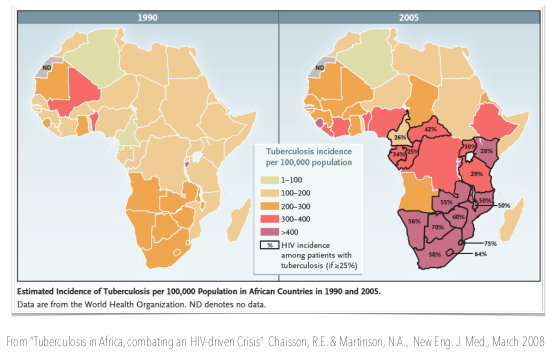
\includegraphics[width=0.6\textwidth]{../lessons/image/11/image001.png}
\caption{\label{fig:11_001} Map of the prevalence of $TB$ for different years (1990 and 2005).}
\end{figure}

This should explain us what is depicted in the map: when people contract HIV, their immune system becomes inactive and consequently Tuberculosis can activate. As one may have understood, HIV has provided much help for the spreading of TB: numbers shown represent the fraction of patients which get both HIV and TB. 
This actually was the \textbf{first example} of \textbf{interaction} of two diseases.


The downside, when \textbf{competition} between diseases may arise, is shown as an example by seasonal influenza. From fig. \ref{fig:11_002} we can see the distribution of the different influenza viruses that are out during a single season. Individuals can be infected by different strains of influenza, therefore the distribution of the prevalence of total infected people is the sum of the values regarding the three strains.

\begin{figure}[h!]
\centering
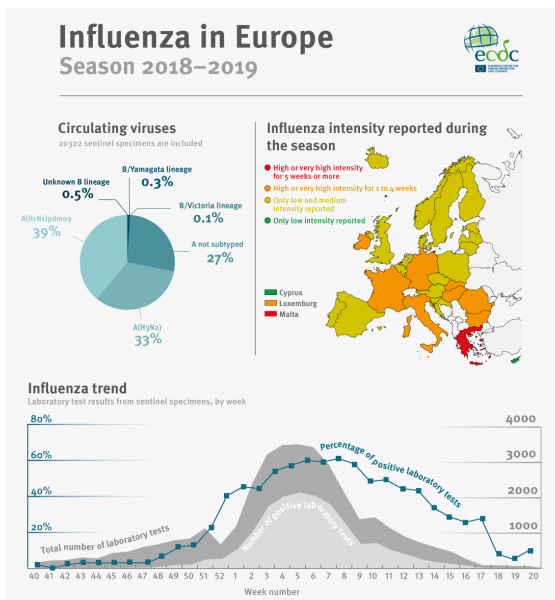
\includegraphics[width=0.6\textwidth]{../lessons/image/11/image002.png}
\caption{\label{fig:11_002} Distribution of different strains of influenza for a single season.}
\end{figure}

It can be shown that our immune system has a sort of \textbf{memory} which provides a \textbf{long lasting} immunity. The main consequence is that if we accidentally get a disease, there is a possibility that we end up not contracting it once again for some time in the future. Moreover, it can provide also a sort of \textbf{cross-immunity} for some other diseases that are similar to the one we contracted, even though our immune systems had never faced them. As one can imagine, this implies that the actual susceptible population is just a reduced fraction of the whole one, and should explain why we do not usually observe influenza pandemics.

However, \textbf{evolution} applies to viruses as well, since they may mutate during time. For instance, HIV is an extremely volatile virus, and is known as one of the fastest evolving entities known: science has categorized different types and subtypes, which are distributed among different regions.

We are now going to focus only on the simplest settings, in which we consider competition and cooperation between only two diseases. We want to discuss how it is possible to \textbf{model} these kind of \textbf{interactions} between diseases/strains and their behaviors. The \textit{simplest solution} to our problem is to \textbf{couple different dynamics}, let us see how.

For instance, the simplest case one can think of is to couple two different diseases whose dynamics are respectively \textbf{SIS} and \textbf{SIS}. We end up having twice the number of states (see fig \ref{fig:11_003}), since we take into account all the possible combinations between compartments. A single node $i$ at time $t$ can be be either one of the following states $\{SS, SI, IS, II,\}$ with its own probability density $\{ [\rho^{SS}]^i_t, [\rho^{SI}]^i_t,[\rho^{IS}]^i_t, [\rho^{II}]^i_t \}$. Therefore, every disease will be defined thanks to its own \textbf{parameters} $\{\beta_1, \beta_2, \mu_1, \mu_2\}$. However, some more are to be introduced, namely the ones that \textbf{encode} the \textbf{interaction} between diseases.

\begin{figure}[h!]
\centering
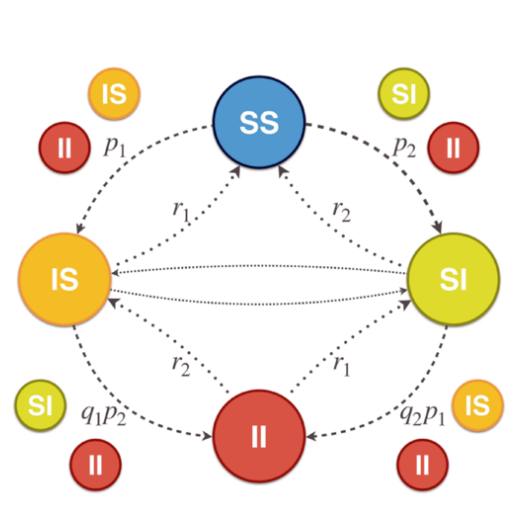
\includegraphics[width=0.3\textwidth]{../lessons/image/11/image003.png}
\caption{\label{fig:11_003} Coupled SIS model and all possible combinations and different transition probabilities between each compartment. }
\end{figure}

As an \textbf{example}, let us discuss one of these models. Let us consider a \textbf{classical heterogeneous mean-field} in which we have \textit{two different diseases} that can spread inside its own network. We are dealing now with the most general case: diseases may spread in different manners and by different means. For example, one may contract a disease orally, while an other one by blood contact. This is the reason why we need to take into account different networks in which diseases spread: every network is peculiar of the disease and can be different one from another, having its own degree distribution or topology. As an example, for $HIV$ we have a network that is defined by its degree distribution $P(k)$, while for $TB$ an other network $P(l)$. However, when dealing with both of them we shall use the joint probability for the two distributions $P(k,l)$.

Recalling now that we are doing a degree based mean field, we are able to divide our network in four different classes according to the compartment they belong to and their degree distributions: $\{SS(k,l),SI(k,l),IS(k,l),II(k,l) \}$. As an example, $SS(k,l)$ is the fraction of nodes of degree $k$ in the first network and $l$ in the second, that is susceptible for both diseases. 

At this point it comes to take into account, and therefore model, the interaction effects between the two diseases (see fig. \ref{fig:11_004}). These interactions may result in three effects:
\begin{itemize}
    \item \textbf{modified susceptibility} $\mathbf{\lambda_a}$: being infected of one diseases makes an individual more $(\lambda_a > 1)$ or less $(\lambda_a < 1)$ probable to be infected by a second one. It is the case for the $HIV$ that increases the probability of contracting $TB$, or for a strain of a seasonal influenza that inhibits individuals to get influenza of another kind 
    \item \textbf{modified infectivity} $\mathbf{\lambda_b}$ once we get infected by one disease, we are less infectious wrt second one
    \item \textbf{modified infectious period} $\mathbf{\eta}$ if we are infected of one disease, it can favor/hinder the recovery from the other disease. As for the second case, it may happen when our immune system is compromised.
\end{itemize}

\begin{figure}[h!]
\centering
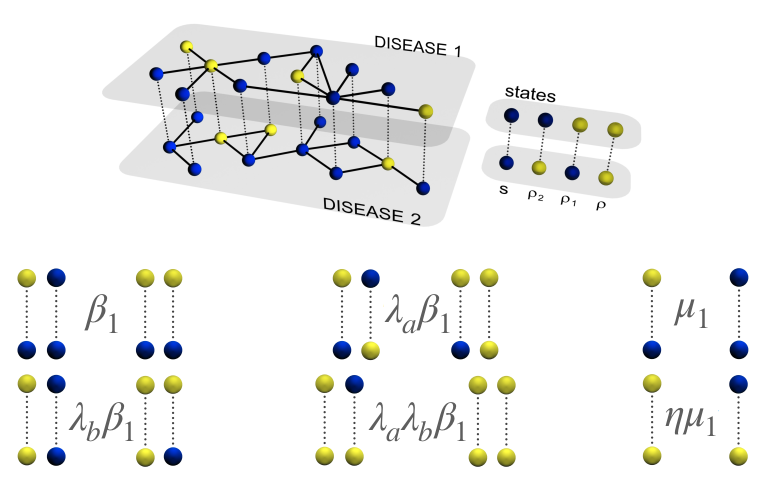
\includegraphics[width=0.6\textwidth]{../lessons/image/11/image004.png}
\caption{\label{fig:11_004} Coupled SIS networks and their effects on each other. }
\end{figure}

In this way we have covered all the possible interactions between diseases, given this simple model. Obviously, the interactions may result in an increasing susceptibility or infectivity, alongwith the tuning aforementioned parameters. Actually, despite in this last model we have introduced all possibilities and cases that we may observe, only a subset of them at time is meaningful and has some sort of biological sense.

Now we may wonder how does the individuals flows between compartments look like:
\begin{align}
    \dot{SS}(k,l) = - (k \sigma_1 + l\sigma_2) SS(k,l) + \mu_1 IS(k,l) + \mu_2 SI (k,l)\\
    \dot{IS}(k,l) = k\sigma_1 SS(k,l) - l \lambda_a \sigma_2 IS(k,l) - \mu_1 IS(k,l) + \eta \mu_2 II(k,l)\\
    \dot{SI}(k,l) = l\sigma_2SS(k,l) - k \lambda_a \sigma_1 SI(k,l) - \mu_2 SI(k,l) + \eta \mu_1 II(k,l)\\
    \dot{II}(k,l) = k\lambda_a\sigma_1SI(k,l) + l \lambda_a \sigma_2 IS(k,l) - (\eta \mu_1 + \eta \mu_2) II(k,l)
\end{align}

Where we have introduced the \textit{infection terms} for the disease 1 and 2. The former can be propagated by both $IS$ and $II$ individuals and the infection term is:
\begin{equation*}
    \sigma_1 = \beta_1 (\Theta_1^{IS} + \lambda_b \Theta_1^{II} )
\end{equation*}
while the disease 2 can be propagated by both $SI$ and $II$:
\begin{equation*}
    \sigma_2 = \beta_2 (\Theta_2^{SI} + \lambda_b \Theta_2^{II} )
\end{equation*}
For the sake of completness we write how $\Theta_i$ look like: they are the probabilities that a link of network either 1/2 points to an infected. For network 1 it holds that:
\begin{equation*}
    \Theta_1^{IS} = \frac{\sum_{k,l} P(k,l) k IS(k,l)}{\sum_{k,l} P(k,l) k}
    \qquad
    \Theta_1^{II} = \frac{\sum_{k,l} P(k,l) k II(k,l)}{\sum_{k,l} P(k,l) k}
\end{equation*}
While for network 2:
\begin{equation*}
    \Theta_2^{SI} = \frac{\sum_{k,l} P(k,l) l SI(k,l)}{\sum_{k,l} P(k,l) l}
    \qquad
    \Theta_2^{II} = \frac{\sum_{k,l} P(k,l) l II(k,l)}{\sum_{k,l} P(k,l) l}
\end{equation*}
The structure is absolutely the same as the one obtained for the one disease framework, and also the procedure to solving these equations. However, we will not start computations and derive all the results since some passages are extremely tedious.

In order to solve these equations, firstly we need to assume that we are in the \textbf{steady state}. Later we are able to write down a couple of self-consistent equations for \( \sigma _1 \) and \( \sigma _2 \), and then solve them by finding the intersection. Finally, the \textbf{epidemic threshold}:
\begin{equation*}
  \beta_1^c( \sigma_2) = \mu_1 \frac{\expval{k}}{\sum_{k,l} P(k,l) k^2 \frac{l^2 \sigma_2^2 \lambda_a^2 \lambda_b + l\sigma_2(\eta \mu_2 \lambda_a  + \lambda_b(\lambda_a \mu_1 + \lambda_a \mu_2)) + \mu_2 ( \eta \mu_1 + \eta \mu_2)}{l^2 \sigma_2^2 \lambda_a \eta + l \sigma_2 (\eta \mu_1 + \eta \mu_2 + \lambda_a \eta \mu_2) + \mu_2(\eta \mu_1 + \eta \mu_2)}}
\end{equation*}
that is quite complex, but the form resembles the one of before.

One should see from the formula that the \textbf{epidemic threshold} of the \textbf{first} disease \textbf{depends} on the \textbf{prevalence of the other}. An other way to see it is that we are assuming that one disease is already there, and then insert a second one and check the effects on the epidemic threshold.

Let us see what happens to the epidemic threshold for different cases. 

For instance, let us consider the 3D epidemic diagram shown for \textbf{cooperating diseases} (see fig. \ref{fig:11_005}) with \( \lambda > 1 \) and \( \eta <1 \).

\begin{figure}[h!]
\centering
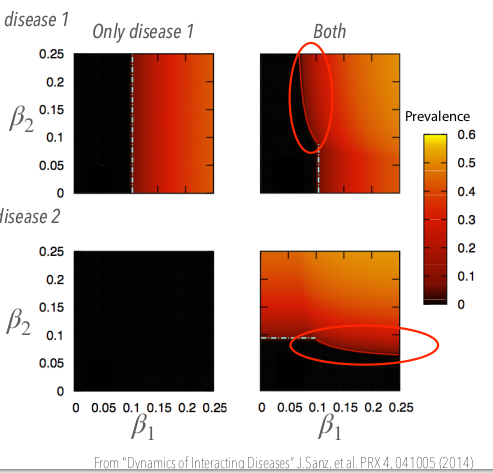
\includegraphics[width=0.6\textwidth]{../lessons/image/11/image005.png}
\caption{\label{fig:11_005} Cooperating diseases, \( \lambda > 1 \) and \( \eta <1 \) }
\end{figure}

If we consider a single disease, one see that we get back the old results (in 2D): since we have not introduced yet a second disease we are not able to see it. On the other hand, if the parameter $\beta_2$ is below the critical threshold, we cannot note any difference and the spreading is the same as before. However, when we overcome the threshold for a disease, one should note the that other's decreases and therefore the disease spreads easier and with a larger prevalence.



The opposite actually occurs when we consider \textbf{competing diseases} (see fig. \ref{fig:11_006}), that is the case \( \lambda < 1 \) and \( \eta >1 \). For either one of them it is more difficult to spread once we have overcome the critical threshold for the other's. This concludes the discussion when taking for heterogeneous mean field degree assumption.

\begin{figure}[h!]
\centering
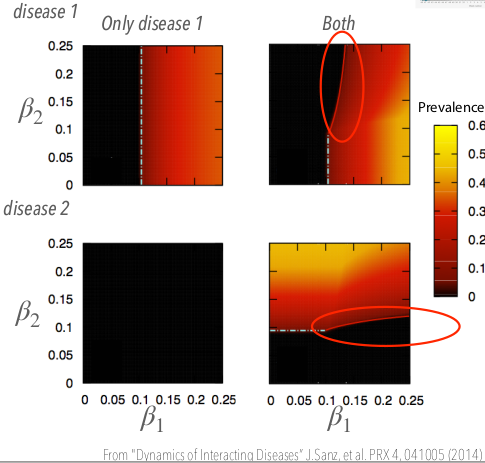
\includegraphics[width=0.6\textwidth]{../lessons/image/11/image006.png}
\caption{\label{fig:11_006} Competing diseases, \( \lambda < 1 \) and \( \eta >1 \) }
\end{figure}

One may wonder now how \textbf{quenched mean-field} equation look like (individual based formulation). For the sake of simplicity we are going to discuss only a single network, and we will take into account only its main effect, that is the one on the \textbf{modified susceptibility}. Also under this assumptions equations $\{[\rho ^{SS}]^{t+1}_i, [\rho ^{SI}]^{t+1}_i, [\rho ^{IS}]^{t+1}_i, [\rho ^{II}]^{t+1}_i \}$ can be written, whose structure is exactly the same one as before for a single disease case. Each term contributes and plays a role in the probabilities \( [\rho ^{IS}]^{t+1}_i, [\rho ^{SI}]^{t+1}_i \). Since these expressions are really long and complex, we are going to skip this part. Nonetheless we will briefly discuss an interesting \textbf{assumption} we make during our computations: we did insert the functions \( f_{SI}, f_{IS} \). It was done to consider the fact that we cannot contract two diseases at the same time, it would be unrealistic. However, if during our simulations it happens, we pick only one disease at random. The function $f_{IS}$ is the following, for the \( [\rho ^{IS}]^{t+1}_i \) expression:
\begin{equation}
    f_{IS} = \frac{q_{IS} (1-0.5 q_{SI})}{q_{IS} (1-0.5 q_{SI}) + q_{SI} (1-0.5 q_{IS})}
\end{equation}
where:
\begin{equation}
    q_{IS} = 1 - \prod_j^N \left[ 1-A_{ij} \beta_1 \left( [\rho ^{IS}]^{t+1}_j + [\rho ^{II}]^{t+1}_j \right) \right]
\end{equation}
and:
\begin{equation}
    q_{SI} = 1 - \prod_j^N \left[ 1-A_{ij} \beta_2 \left( [\rho ^{SI}]^{t+1}_j + [\rho ^{II}]^{t+1}_j \right) \right]
\end{equation}

These equations can be solved numerically by iteration as we did for the single disease scenario. One should have noticed that when \( \lambda = 1 \) we get back to the classical case. Let us see now what happens when the two diseases \textbf{cooperate}. Recalling that:
\begin{equation}
    \rho = \frac{1}{N} \sum_{i=1}^N (\rho_i^{IS} + \rho_i^{SI} + \rho_i^{II})
\end{equation}
If the probability of getting the disease is \( \lambda = 2 \) one can see in fig. \ref{fig:11_007} that the curve becomes steeper and, as $\lambda$ increases more this behavior accentuates even more and looks like exploding. Moreover one should note that, despite the infectivity $\beta$ is exactly the same, the prevalence $\rho$ shows some discontinuities that becomes larger as more the two diseases cooperate more and more.

\begin{figure}[h!]
\centering
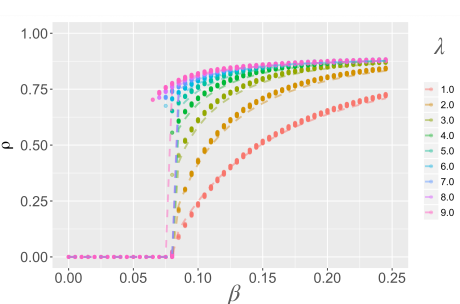
\includegraphics[width=0.6\textwidth]{../lessons/image/11/image007.png}
\caption{\label{fig:11_007} Cooperating diseases, numerical simulations results for different $\lambda$. }
\end{figure}

Let us now see what happens when two diseases \textbf{compete}. The resulting effect is the so called full \textbf{cross-immunity}: once we contracted a disease we cannot get the other one. Accordingly the prevalence is:
\begin{equation}
    \rho = \frac{1}{N} \sum_{i}^N (\rho_i^{SI} + \rho_i^{IS})
\end{equation}

As expected, the prevalence shown in left figure \ref{fig:11_009} does not change at all and is the same as before. While, plotting the difference $|\rho^{IS} - \rho^{SI}|$ we observe some oscillations in values slightly after the critical threshold. This is explained by saying that only a disease can survive, and which is given by chance, being the two symmetrical (see right fig \ref{fig:11_009}). As $\beta$ increases, we see as the difference approaches zero: both of them here survive each with the same prevalence. That is to say that a half of infected population has contracted a disease, while the other half the second one. For large $\beta$ we see as the two diseases coexist.

\begin{figure}[h!]
\begin{minipage}[c]{0.5\linewidth}
\centering
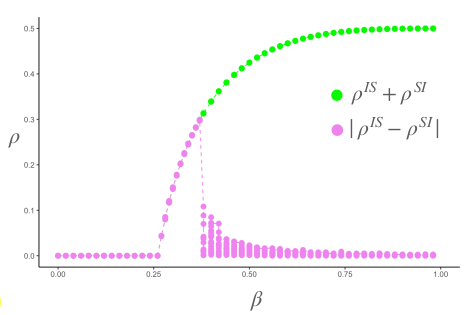
\includegraphics[width=1\textwidth]{../lessons/image/11/image008.png}
\end{minipage}
\begin{minipage}[]{0.5\linewidth}
\centering
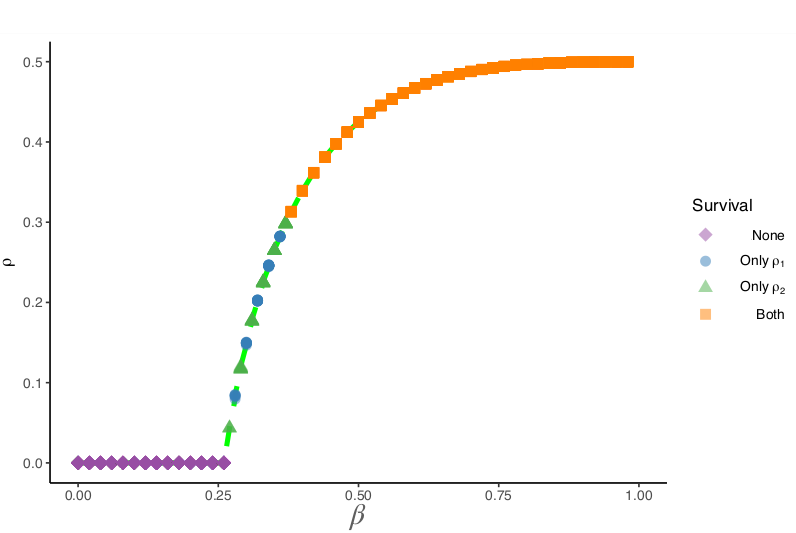
\includegraphics[width=1\textwidth]{../lessons/image/11/image009.png}
\end{minipage}
\caption{\label{fig:11_009} \textbf{Left:} Competing diseases, numerical simulations results. \textbf{Right:} Competing diseases, numerical simulations results with particular attentions to the \textbf{survival disease}. In the intermediate regime, the survivor is chosen by chance. }
\end{figure}

This system actually can be studied also in terms of its dynamics. We start by noting that it has two stable points. They might for instance coincide in the origin in the $(\beta_1, \beta_2)$ space: here obviously both of them are absent. We can continuously move these points and increase $(\beta_1, \beta_2)$ that are not anymore degenerate: the system will settle in either one of these attractors after some time. Later, when we have overcome a certain threshold, the stable points will again coincide and find ourselves exactly in the middle. Here, both diseases are coexisting with exactly the same prevalence. However if we introduce a slight difference between them, i.e. they are not symmetrical anymore, the stable point will not be in the middle anymore but slightly move according to what we have changed.

\begin{figure}[h!]
\centering
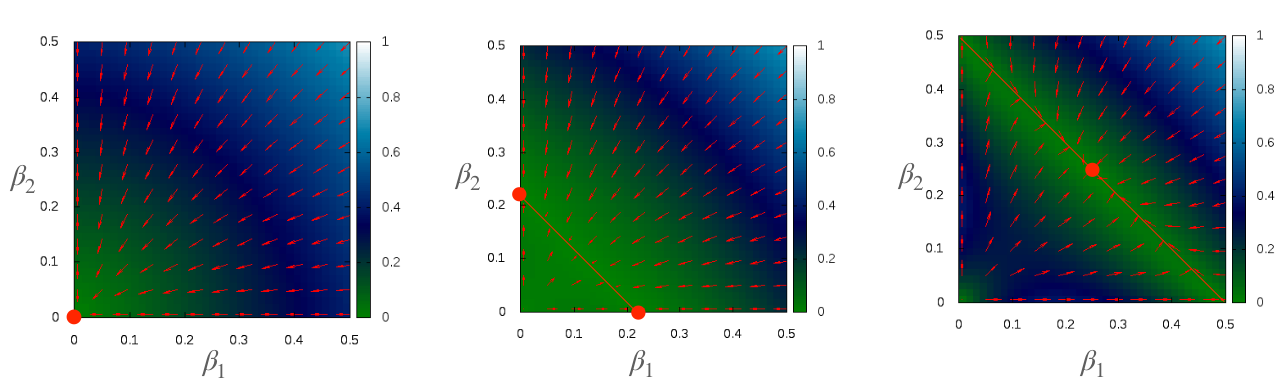
\includegraphics[width=1.0\textwidth]{../lessons/image/11/image010.png}
\caption{\label{fig:11_010} Competing diseases, manyfold that describes the dynamics of the prevalence according to different values of $\beta_1$ and $\beta_2$. }
\end{figure}

\chapter{Spreading in social systems}

Let us now discuss about how we can apply the epidemic models we have studied so far to other scenario, especially in \textbf{social systems}. Indeed, spreading of information inside social systems shares many similarities with epidemic spreading (i.e. “viral information”). This is why one can find a huge literature about these topics, where \textbf{epidemic models} are \textbf{adapted} in order to include also \textit{social aspects}.

However, there are also some differences: the \textbf{communication aspect} actually behaves in its own way and leads to some effects that cannot be totally included in simple epidemic models. In social contexts things are a bit more complex:
\begin{itemize}
\item \textbf{information transmission} is an \emph{intentional} act for both sender and receiver;

\item often \textbf{beneficial} for senders and receivers (e.g. \textbf{reinforcement}), that is to say we are "invited" to acquire more information while feeling like spreading it. Indeed, the information can be replicated by different sources: for instance we often see the same information different times in different places;

\item influenced by cognitive and \textbf{psychological factors};

\item content of information matters (e.g. \textbf{homophily}), so we tend to cluster among people that share the same knowledge or type of information.

\end{itemize}


According to these last properties, there are different instances of\textbf{spreading}, and a single one can be \textbf{defined} as:
\begin{itemize}
\item \textbf{simple contagion} if there is \textbf{no memory}, \textbf{no reinforcement} 
\item \textbf{complex contagion} if \textbf{multiple exposures} and reinforcement are involved, i.e. we keep trace of past interactions that can be either independent of each other.

\end{itemize}

In addition, we shall introduce the so called \textbf{threshold models},that present some sort of threshold effect. Empirically, we may say that if only few friends bought a certain product we would not feel like buying it, as it would be if nearly half or hall of them have bought it. In the old fashioned models, when we were susceptible, our infected neighbours tried to infect us along with a certain probability. But, in this case, if our \textbf{neighbours number} is \textit{lower} than a certain \textit{threshold}, we \textbf{cannot be infected} by them. Conversely, if their number is either equal or above that threshold we are going to change our state.

In particular, threshold models lead to \textbf{information cascades}, that is to say that if someones acquires some information then he will start spreading it to other people. In turn, they will keep on sharing it until it will have reached a huge amount of individuals as in a sort of $cascade$. 


\section{Complex contagion}

We want now to generalize what we have told so far, and introduce some sort of more abstract model which is able to mediate between complex and simple contagions.

The main \textbf{assumptions} we will make for such general contagion model, able to reproduce both simple and complex contagions, are the following:
\begin{itemize}
\item we will assume to deal with \textbf{well-mixed population};

\item we will introduce the usual three \textbf{compartments} as in the $SIR$ models: thus we will end up with different classes \( S \) \textit{(susceptible)}, \( I \) \textit{(infected)} and \( R \) \textit{(recovered)} of individuals;

\item we will \textbf{keep trace of past interactions} up to time $T$, since we want to take into account the effects given by different exposures in different period of times;

\item we will change the \textbf{way information is spread}: given a successful interaction with an infected $j$, a susceptible individual $i$ gets a “dose” of infection $d_i(t)$. This is done to take into account that the more we see a certain information, the more likely it will be spread in the future;

\item Once the \textbf{accumulated dose} $D_i(t) = \sum_{t'=t-T+1}^{t} d_i(t')$ exceeds a fixed threshold $d_i^*$, then the $i$-th susceptible individual becomes in turn infected.

\end{itemize}

As one can see, we actually started from a $SIR$ dynamics and applied some changes to it, in order to create the general contagion model that can be applied to social networks. 
Whereas, regarding the dynamics of the \textbf{infection} process:

\begin{itemize}
\item at each time step \( t \):
        \begin{itemize}
        \item each individual $i$ contacts a random individual $j$;
        \item if $i = S$ and $j = I$, with probability $p$, individual $i$ gets a “dose” of infection $d_i(t)$ that is distributed according to a dose size distribution $f(d)$;
        \item with probability $1-p$, that is to say if the contact has not been successful, $d_i(t)=0$.
        \end{itemize}
\item each individual keeps trace of the doses acquired in $T$ timesteps via the \textbf{“cumulative” dose}: $D_i(t) = \sum_{t'=t-T+1}^{t} d_i(t')$.

\item if the cumulative dose $D_i(t)$ is larger than the individual threshold $d_i^*$, individual $i$ gets infected.
\end{itemize}

As for the \textbf{recovery} process, the dynamics is more or less resembling the classical dynamics:
\begin{itemize}
\item if $D_i(t)$ gets below $d_i^*$, $i$ recovers with probability $r$;
\end{itemize}

If one would like to create a more complex model, it is also possible to add an $R \rightarrow S$ transition that occurs with probability $r'$. This could be done to simulate an \textbf{SIRS} model with reinfection dynamics. The limiting case, namely the one with $r = 1$ and $r' = 1$, we end up again having an SIS-like dynamics.


Having said so, let us now summarize the main parameters we introduced so far:
\begin{itemize}
\item \( p \) and \( r \) are \textbf{infection} and \textbf{recovery} probabilities. They actually play the same role as \( \beta  \) and \( \mu  \) in the epidemiological models;
\item $d_i(t)$ \textbf{“dose” per infection}, which distributes according to $f(d)$;
\item \( d_i^* \) \textbf{threshold}, in turn distributed following \( g(d^*) \).
\end{itemize}

Note that \( f(d) \) and \( g(d^*) \) can be \textit{any} distributions. By varying them we can reproduce different behaviors, i.e. obtain different dynamics. However, with specific choices of $p$, $f(d$) and $g(d^*)$, it is possible to tune the effects of the threshold dynamics to our system. For instance, for either low or null threshold (or relatively high-valued doses distributions) we observe a dynamic really resembling the ones we have studied so far. Conversely, we may end up to models where the "threshold dynamics" is the one that characterize and strongly determines the behavior of the system.


Let us now \textbf{formalize} mathematically what we have said up to now and finally try to solve it. Firstly, let us define the \textbf{probability} for an \textbf{individual} with \( K < T  \) contacts to be \textbf{infected} as:
\begin{equation}
  P_{inf} (K) = \sum_{k=1}^{K} \begin{pmatrix}
  K \\
  k
  \end{pmatrix}
  p^k (1-p)^{K-k} P_k
\end{equation}
Let us discuss the single terms. \( p^k (1-p)^{K-k} \) is the probability for the contact to be successful. Note as it a \textit{Bernoulli distribution} with \( K \) trials and \( k \) successes. This is multiplied by the Binomial coefficient that takes into account all the possible combinations of $k$ successes in $K$ trials \( \begin{pmatrix}
K \\
k
\end{pmatrix}  \) and, finally, it is multiplied by the factor \( P_k \).
In particular  \( P_k \) is the \textit{average fraction of infected individuals} after having received \( k \) doses in \( T \) time steps:
\begin{equation}
  P_k = \int_{0}^{\infty }  \dd[]{d^*} g(d^*) P \qty(\sum_{i=1}^{k} d_i \ge d^*  )
\end{equation}
which one can easily note, do depend on the thresholds. Indeed, \(  P \qty(\sum_{i=1}^{k} d_i \ge d^*  )  \) is the probability that \( k \) doses exceed \( d^* \).



This model can actually be solved numerically for any distribution of $f(d)$ and $g(d^*)$. However, for some specific cases we can recover classical dynamics. Indeed let us consider:
\begin{itemize}

\item if the probability of a successful contact \( p<1 \), the dose has a fixed size $f(d) = \delta(d-1)$ and fixed threshold $g(d^*) = \delta(d^*-1)$, we observe \textbf{epidemic spreading} where interactions are independent (see fig. \ref{fig:11_1}). In particular, all contacts share the same infection probability and the threshold is $d^* = 1$, i.e. one successful contact is enough to contract the disease. In addition, if we want to recover an SIS dynamics, we must constrain the dose to be the same for everyone and the threshold to be unique

\begin{figure}[h!]
\centering
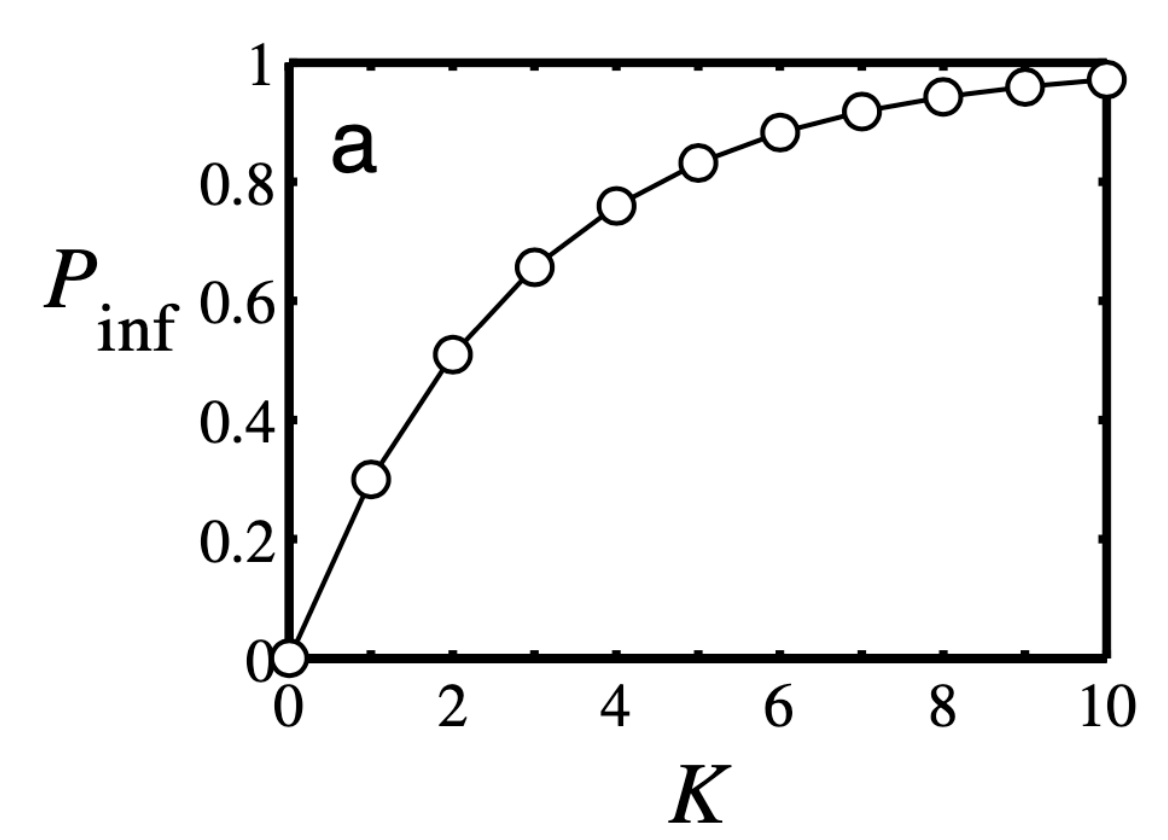
\includegraphics[width=0.4\textwidth]{../lessons/image/11/1.png}
\caption{\label{fig:11_1} Generalized Complex Contagion model: epidemic spreading.}
\end{figure}


\item if the probability of a successful contact \( p=1 \), the dose has fixed size $f(d) = \delta(d-1)$ and fixed threshold $g(d^*) = \delta(d^*-5)$, we obtain a \textbf{deterministic threshold model} (see fig. \ref{fig:11_2}). In particular, we arbitrarily fixed the threshold at \( d^*=5 \), that is to say that we need at least 5 encounters to be infected (they do happen with $p=1$, so every contact is actually successful!). Hence, despite the dose size is exactly the same as before being the distribution peaked in 1, in this case we actually need more than a single contact to contract the disease.\footnote{for instance 5 friends that show to me the same information.}

\begin{figure}[h!]
\centering
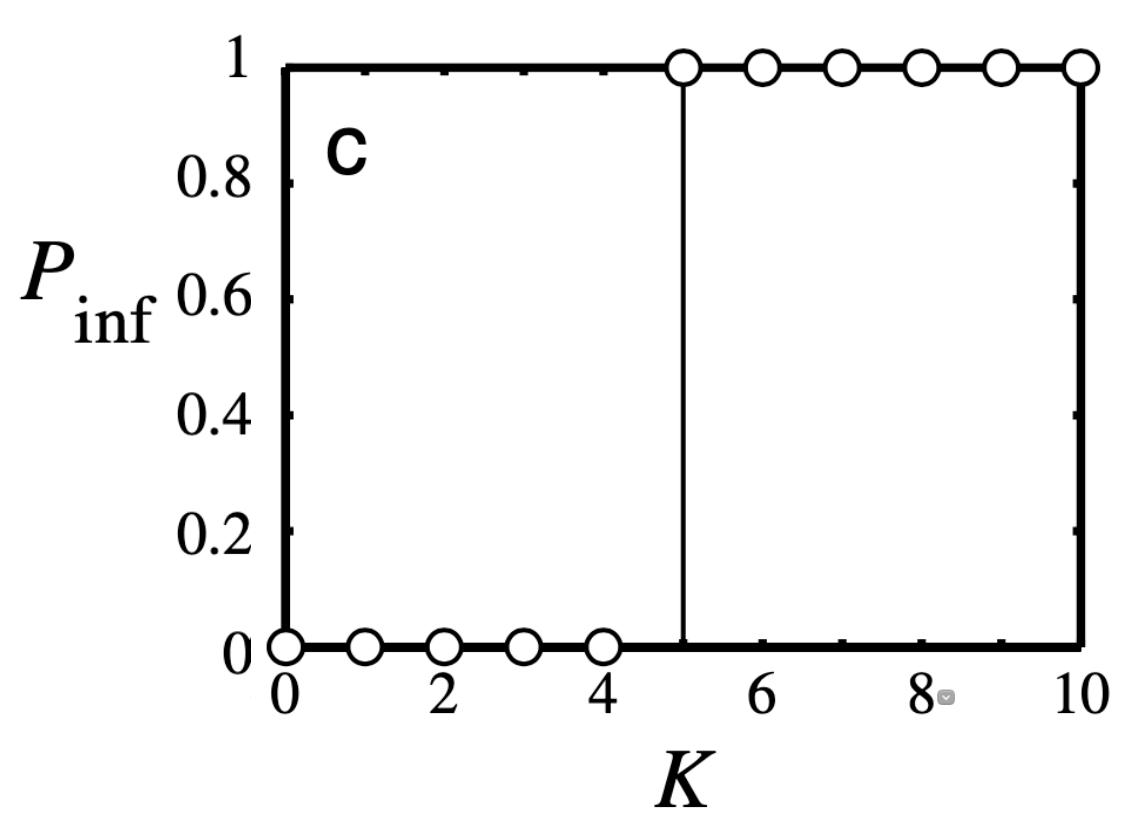
\includegraphics[width=0.4\textwidth]{../lessons/image/11/2.png}
\caption{\label{fig:11_2} Generalized Complex Contagion model: deterministic threshold model.}
\end{figure}

\item if the probability of a successful contact \( p=1 \) , the dose size $f(d)$ distributes log-normally and the threshold is fixed $g(d^*) = \delta(d^*-5)$ we obtain the so called \textbf{stochastic-threshold model} (see fig. \ref{fig:11_3}). In particular, we observe that the threshold is still fixed at \( d^*=5 \), but now the “dose” per successful contact varies.
In this case we assume contacts to not be equal among them, so despite the threshold being fixed, the dose size is actually different.\footnote{for instance we may trust some friends/people more than others, hence we give more importance to their information rather than acquaintances' one.} 

\begin{figure}[h!]
\centering
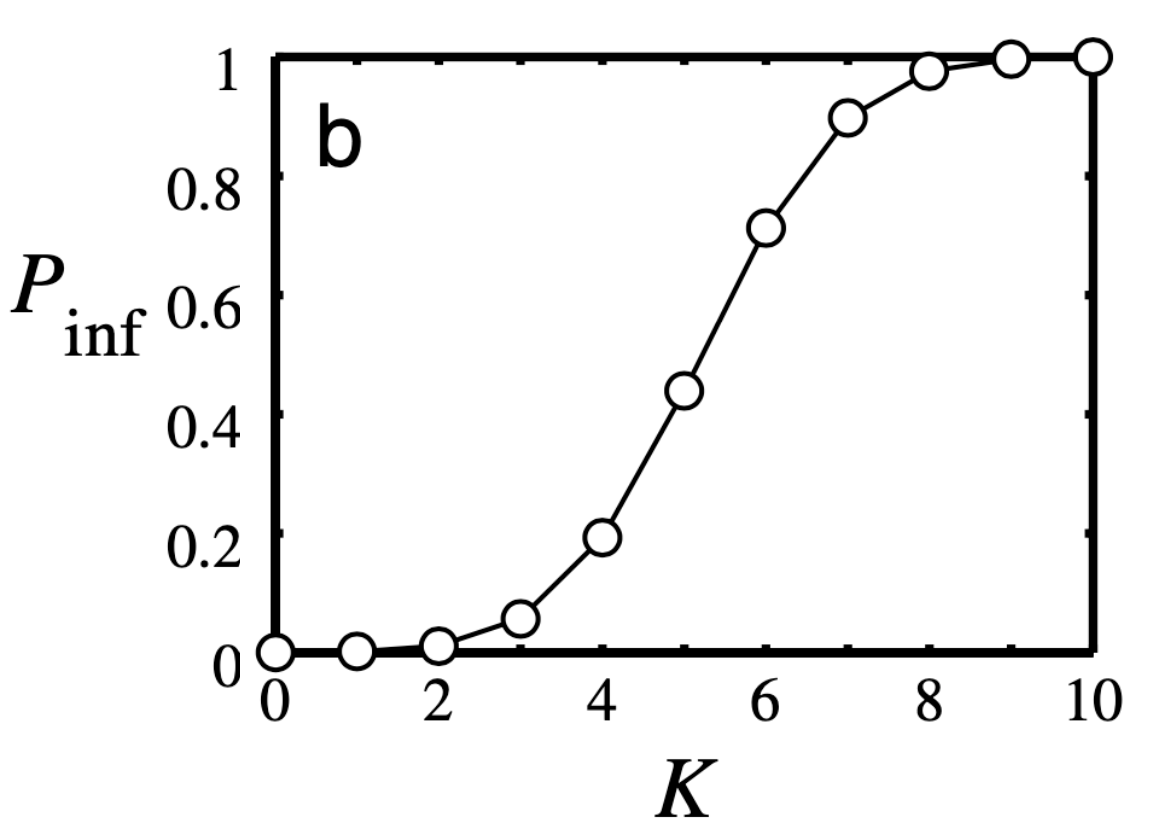
\includegraphics[width=0.4\textwidth]{../lessons/image/11/3.png}
\caption{\label{fig:11_3} Generalized Complex Contagion model: stochastic threshold model.}
\end{figure}

\end{itemize}






\section{Applications to Online Social Networks}

We want to apply our framework to real social networks, thus we want to understand how hashtags or memes spread in online social communities. Let us consider the analysis of real data extracted from Twitter. In the latter we may have different types data: however we are going to focus only on retweets (RT) and mentions (@) that contribute to the diffusion of hashtags in different communities. In particular we want to see whether the structure, namely reinforcement and homophily, inside communities does have a role in the spreading.

To quantify the fraction of information that flows inside and outside of a community, we will introduce the following weights:
\begin{itemize}
\item \( \expval{w_\circlearrowright}_c  \) is the average weight (number of tweets) per link inside the community;

\item \( \expval{w_\curvearrowright}_c  \) is the average weight (number of tweets) per link outside the community.
\end{itemize}
And the same for users activity:
\begin{itemize}
\item \( f_\circlearrowright \) is the fraction of activity inside the community;

\item \( f_\curvearrowright  \) is the fraction of activity outside the community.
\end{itemize}

If information in Twitter spread like a \emph{simple contagion}, there should not be any noticeable differences in the spreading process inside and outside a community (e.g. we observe \emph{no reinforcement}). Conversely, if we saw that the average weights inside a community would be larger than outside ones, actually we should take into account some sort of reinforcement.

In Fig. \ref{fig:11_4} we can see the results showing the average weight inside and outside a community. They are actually pretty similar, but if we take a look more closely, we may notice that the averages for spreading inside a community are little higher, therefore we can conclude that homophily and reinforcement do play a role.

\begin{figure}[h!]
\centering
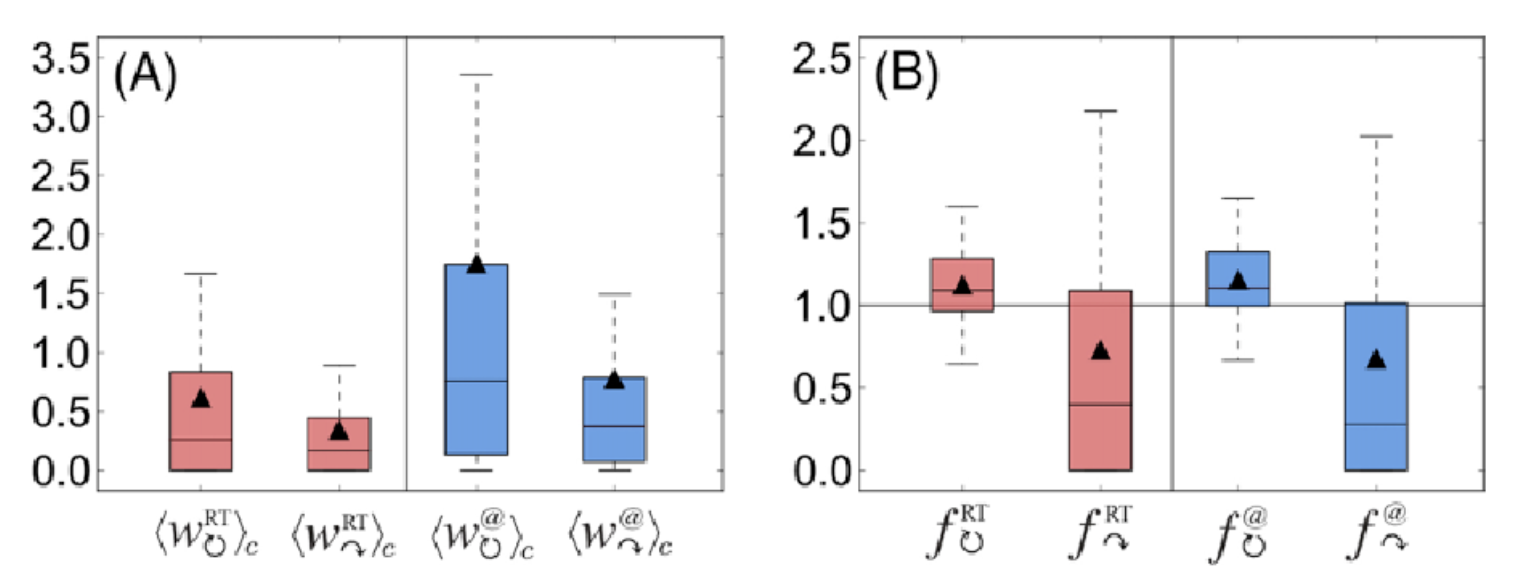
\includegraphics[width=0.8\textwidth]{../lessons/image/11/4.png}
\caption{\label{fig:11_4}  Spreading inside a community is favored (effects of homophily and reinforcement are noticeable).}
\end{figure}

To clarify this last point, we introduce a new metric on the level of single hashtags (\( h \)). Hence we measure the average popularity of an hashtag inside and outside a community, i.e. for every hashtag we measure the popularity that a tweet exploiting the latter had. In particular, for each hashtag:
\begin{itemize}

\item we measure the \textbf{usage dominance} $r(h)$. This is the ratio of tweets produced inside the “main” community of $h$ and the total number of tweets containing $h$, namely $T(h)$. We expect that this metric is low for viral spreading and high for complex contagions;

\item we measure the \textbf{usage entropy} \( H(h) \): how \( h \) is distributed across communities. It is high for viral spreading and low for complex contagion;

\item we measure the \textbf{average exposure} $N(h)$: which is the average number of exposures needed to adopt hashtag $h$. It is low for viral spreading and high for complex contagion.

\end{itemize}

In order to analyze it, we use some reference models (4 models \( M_{1, \dots,4} \)) in order to represent different baseline behaviors (see Fig. \ref{fig:11_5} for more details):

\begin{itemize}
\item the simplest model is $M_1$ where, for a given hashtag \( h \), we randomly sample the number of tweets or users using the averages we have from real data (i.e. we assume that data is extracted at random). In such way, we can obtain some sort of \textbf{average behavior} for all the hashtags where we do not consider any community, neither network structure;

\item the second model $M_2$ is simply an epidemic model. In particular, it takes into account the \emph{network structure} while neglecting social reinforcement and homophily.  Each hashtag therefore starts from some random users (the "seed") and, at each timestep, it spreads to other users according to a certain probability. This is indeed a reference model for \textbf{simple contagion};

\item However we can have more complex models which can take into account \emph{network structure}, \emph{reinforcement} and \emph{homophily}. This is a reference model for \textbf{complex contagion}.
\end{itemize}

\begin{figure}[h!]
\centering
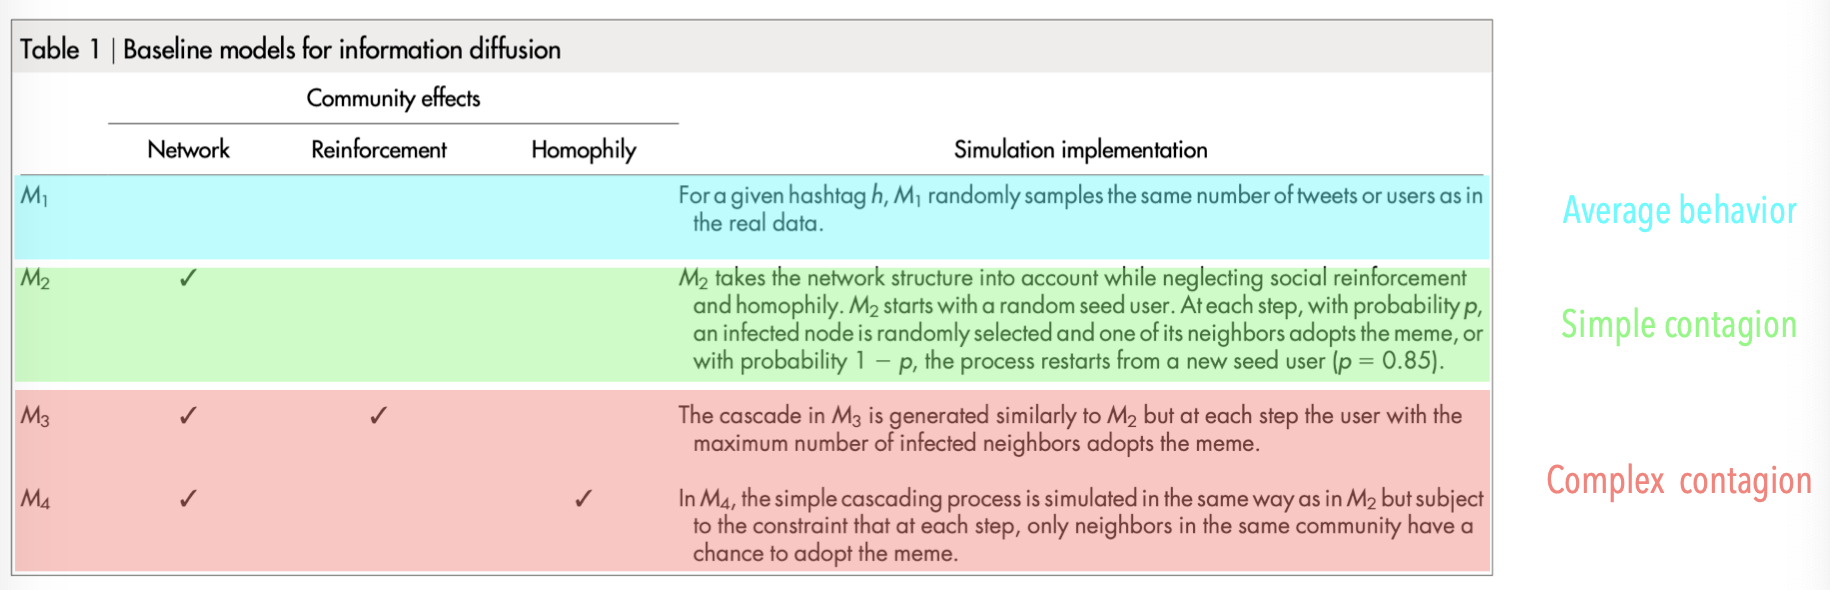
\includegraphics[width=0.9\textwidth]{../lessons/image/11/5.png}
\caption{\label{fig:11_5} Reference models for information spreading in online social networks.}
\end{figure}

Let us consider Fig. \ref{fig:11_6} where we can see \( r(h) \), \( H(h) \) and \( N(h) \) in function of the number of tweets \( T \) and number of users \( U \).
Black lines represent the real data, while the dashed line represents the theoretical results returned from model \( M_1 \) (average behavior), whereas the red square \( M_2 \) (simple contagion model) and last the blue and green lines given by models \( M_3 \) and \( M_4 \) (complex contagion).

One can note as popular (in grey) and not popular hashtags do result in two different behaviors, therefore can be easily distinguished and separated into two different classes.
In particular, it holds that:
\begin{itemize}
\item popular hashtags (large $T$ and $U$) spread like epidemics (viral);
\item less popular ones follow a complex contagion.
\end{itemize}

\begin{figure}[h!]
\centering
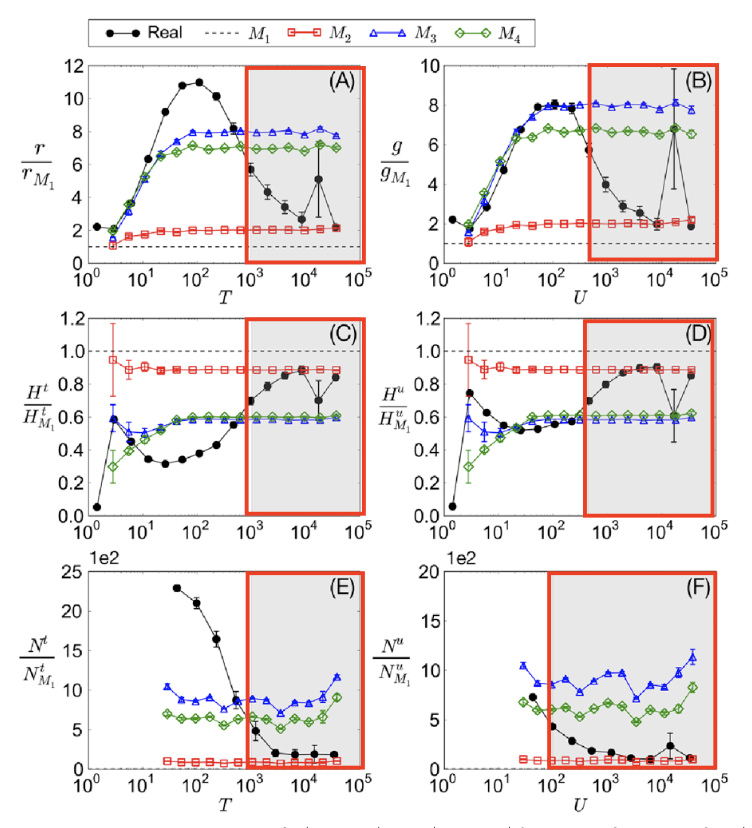
\includegraphics[width=0.9\textwidth]{../lessons/image/11/6.png}
\caption{\label{fig:11_6} Results of information spreading in online social networks.}
\end{figure}


\end{document}
